\bookchapter{What can AI do? An overview}\label{ch:ai1}

\section*{Explanation}
``Artificial intelligence'' is a big word for many different ideas. A chess program from 1997, the spam filter in your mail, the camera of a robot that finds the ball and a chatbot all count as AI, but they work in completely different ways. This chapter is a map of the landscape. You will see the main families of methods, what kind of problem each one solves, and where the neural networks of this book fit in.

\begin{center}
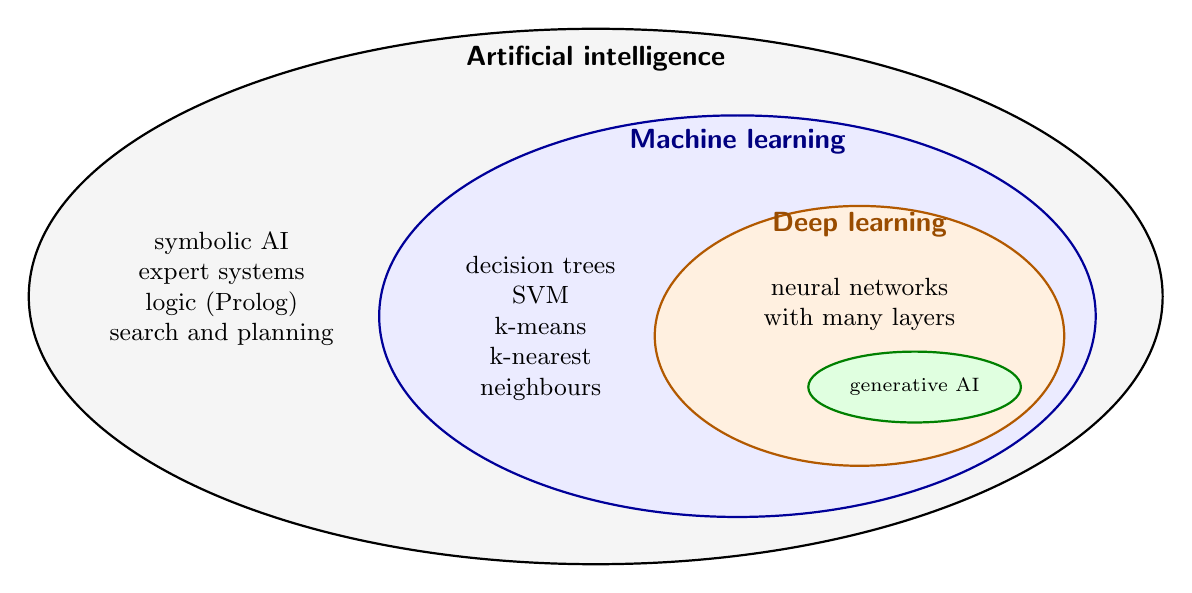
\begin{tikzpicture}
  \fill[gray!8] (0,0) ellipse (7.2cm and 3.4cm);
  \draw[thick] (0,0) ellipse (7.2cm and 3.4cm);
  \node[font=\sffamily\bfseries,anchor=north] at (0,3.3) {Artificial intelligence};
  \node[font=\small,align=center] at (-4.75,0.1) {symbolic AI\\expert systems\\logic (Prolog)\\search and planning};
  \fill[blue!8] (1.8,-0.25) ellipse (4.55cm and 2.55cm);
  \draw[thick,blue!60!black] (1.8,-0.25) ellipse (4.55cm and 2.55cm);
  \node[font=\sffamily\bfseries,blue!50!black,anchor=north] at (1.8,2.25) {Machine learning};
  \node[font=\small,align=center] at (-0.7,-0.4) {decision trees\\SVM\\k-means\\k-nearest\\neighbours};
  \fill[orange!12] (3.35,-0.5) ellipse (2.6cm and 1.65cm);
  \draw[thick,orange!70!black] (3.35,-0.5) ellipse (2.6cm and 1.65cm);
  \node[font=\sffamily\bfseries,orange!60!black,anchor=north] at (3.35,1.2) {Deep learning};
  \node[font=\small,align=center] at (3.35,-0.1) {neural networks\\with many layers};
  \fill[green!12,draw=green!50!black,thick] (4.05,-1.15) ellipse (1.35cm and 0.45cm);
  \node[font=\scriptsize,align=center] at (4.05,-1.15) {generative AI};
\end{tikzpicture}
\captionof{figure}{The landscape of AI. Machine learning is one part of AI, deep learning (neural networks) is one part of machine learning, and generative AI is one important application of deep learning.}\label{fig:ai1_nested}
\end{center}

\begin{keyidea}[AI vs. machine learning vs. deep learning]
\textbf{Artificial intelligence} is every method that lets a computer do something that normally needs human intelligence. \textbf{Machine learning} (ML) is the part of AI in which the computer \emph{learns from data} instead of following rules that a programmer wrote. \textbf{Deep learning} is the part of machine learning that uses neural networks with many layers.
\end{keyidea}

\section*{Classical AI: rules and logic}
The oldest AI does not learn at all. People write down their knowledge as rules and the computer applies them. This is called \textbf{symbolic AI}.

\textbf{Expert systems.} An expert system stores the knowledge of an expert as \texttt{IF}\,--\,\texttt{THEN} rules. A very simple behaviour of a soccer robot:
\begin{verbatim}
facts = {"ball_visible": True, "ball_distance": 2.5, "battery": 80}

rules = [
    ("low battery", lambda f: f["battery"] < 10, "go to charger"),
    ("ball far",
     lambda f: f["ball_visible"] and f["ball_distance"] > 1.0,
     "walk to ball"),
    ("ball near",
     lambda f: f["ball_visible"] and f["ball_distance"] <= 1.0,
     "kick the ball"),
    ("no ball", lambda f: not f["ball_visible"], "turn and search"),
]

for name, condition, action in rules:
    if condition(facts):
        print(name, "->", action)
        break
\end{verbatim}
The program prints \texttt{ball far -> walk to ball}. Expert systems are transparent (you can read why a decision was made) and need no data, but somebody must write \emph{all} rules, and the rules cannot handle situations that nobody thought of. Many robots still use rules for the high-level behaviour (state machines and behaviour trees, see Part~XI).

\textbf{Logic programming.} In a language such as \textbf{Prolog} you state \emph{facts} and \emph{rules} and then ask \emph{questions}. The computer finds the answers by logical reasoning:
\begin{verbatim}
teammate(anna, ben).
teammate(anna, clara).
free(ben).

can_pass(X, Y) :- teammate(X, Y), free(Y).

?- can_pass(anna, Who).
Who = ben.
\end{verbatim}
The rule reads: ``$X$ can pass to $Y$ \emph{if} $Y$ is a teammate of $X$ \emph{and} $Y$ is free.'' Anna cannot pass to Clara because the fact \texttt{free(clara)} is missing.

\textbf{Search and planning.} Another classical family finds a sequence of actions by searching through possibilities, for example the shortest path across the field with the A$^*$ algorithm, or the best move in chess. The robot uses it for path planning.

\begin{aibox}
Classical AI is not ``old and useless''. Rules and search are exact, fast and easy to check, which matters for safety. A strong RoboCup robot typically combines both worlds: learned perception (neural networks) and hand-written decision logic.
\end{aibox}

\section*{Machine learning: learning from data}
In machine learning the programmer does not write the rules. Instead we collect \textbf{data}, choose a \textbf{model} with adjustable numbers, and let an algorithm adjust the numbers so that the model fits the data. This is the idea of the tiny neural network of Chapter~\ref{ch:nn}. Before neural networks became so successful, several other models were (and still are) very popular. They work on tables of numbers (\textbf{features}).

\subsection*{Decision trees}
A \textbf{decision tree} asks a series of yes/no questions. The questions are chosen automatically from the data. Suppose a robot has recorded ten situations, with the distance $d$ to the goal in metres, whether an opponent stands in front, and what the better action was:

\begin{center}
\renewcommand{\arraystretch}{1.15}
\begin{tabular}{c|cccccccccc}
sample & 1 & 2 & 3 & 4 & 5 & 6 & 7 & 8 & 9 & 10\\ \hline
$d$ (m) & 1.5 & 2.0 & 2.5 & 3.0 & 3.5 & 4.5 & 5.0 & 6.0 & 2.0 & 1.0\\
opponent in front & no & yes & no & no & yes & no & no & yes & no & yes\\
best action & shoot & pass & shoot & shoot & pass & pass & pass & pass & shoot & pass
\end{tabular}
\end{center}
How does the algorithm choose a question? It measures how \emph{mixed} the groups are after a split with the \textbf{Gini impurity}
\[
G=1-\sum_{c}p_c^{\,2},
\]
where $p_c$ is the share of class $c$ in the group. A pure group has $G=0$, two classes of equal size give $G=0.5$. In our data $4$ of $10$ samples are ``shoot'' and $6$ are ``pass'', so $G=1-(0.4^2+0.6^2)=0.48$. The question ``opponent in front?'' gives two groups. With an opponent: $4$ samples, all ``pass'', $G=0$. Without an opponent: $6$ samples ($4$ shoot, $2$ pass), $G=1-(\frac46)^2-(\frac26)^2=0.444$. The weighted impurity is $\frac{4}{10}\cdot0+\frac{6}{10}\cdot0.444=0.267$, much better than $0.48$. The question ``$d\le3.25$\,m?'' happens to give the same value. Take the first one as the root and repeat inside the impure group. There, ``$d\le3.75$\,m?'' separates the classes perfectly.

\begin{center}
\begin{tikzpicture}[node distance=1.2cm, q/.style={draw,rounded corners,fill=blue!8,thick,align=center,font=\small,minimum height=0.9cm}, leaf/.style={draw,rounded corners,thick,align=center,font=\small,minimum height=0.9cm,minimum width=2.4cm}]
  \node[q] (root) at (0,0) {opponent in front?};
  \node[leaf,fill=orange!15] (pass1) at (-3.6,-2.2) {\textbf{pass}\\{\scriptsize 4 samples}};
  \node[q] (d) at (3.0,-2.2) {$d\le3.75$\,m?};
  \node[leaf,fill=green!15] (shoot) at (0.8,-4.4) {\textbf{shoot}\\{\scriptsize 4 samples}};
  \node[leaf,fill=orange!15] (pass2) at (5.2,-4.4) {\textbf{pass}\\{\scriptsize 2 samples}};
  \draw[-{Stealth},thick] (root) -- node[above left,font=\scriptsize]{yes} (pass1);
  \draw[-{Stealth},thick] (root) -- node[above right,font=\scriptsize]{no} (d);
  \draw[-{Stealth},thick] (d) -- node[above left,font=\scriptsize]{yes} (shoot);
  \draw[-{Stealth},thick] (d) -- node[above right,font=\scriptsize]{no} (pass2);
\end{tikzpicture}
\captionof{figure}{The decision tree learned from the ten samples. A new situation is classified by following the questions from the top to a leaf.}\label{fig:ai1_tree}
\end{center}
Decision trees are easy to read and fast. Many trees together (a ``random forest'') are often very accurate on tables of numbers.

\subsection*{Support vector machines}
A \textbf{support vector machine} (SVM) separates two classes with a straight line (in 3D a plane). Many lines are possible, so it chooses the one with the largest \textbf{margin}, the empty band between the classes. The points that touch the band are the \textbf{support vectors}. For the points in Figure~\ref{fig:ai1_svm} the best line is $\tfrac23x_1+\tfrac23x_2-3=0$, i.e.\ $x_1+x_2=4.5$. The margin lines are $x_1+x_2=3$ and $x_1+x_2=6$. The width of the band is $2/|\vv w|=2/0.943=2.12$, where $\vv w=(\frac23,\frac23)$. A new point is classified by the sign of $\vv w\cdot\vv x+b$. With a trick (the ``kernel'') an SVM can also separate classes that need a curved boundary.

\begin{center}
\begin{tikzpicture}
\begin{axis}[grn, width=8cm,height=7cm, xmin=0,xmax=6,ymin=0,ymax=6, xtick={0,...,6}, ytick={0,...,6}, xlabel={$x_1$}, ylabel={$x_2$}, axis lines=left, xlabel near ticks, ylabel near ticks]
  \addplot[blue!60!black,very thick,domain=0:6]{4.5-x};
  \addplot[blue!60!black,dashed,domain=0:6]{3-x};
  \addplot[blue!60!black,dashed,domain=0:6]{6-x};
  \addplot[only marks,mark=*,mark size=2.6pt,red!80!black] coordinates {(1,1)(2,1)(1,2)};
  \addplot[only marks,mark=square*,mark size=2.6pt,green!50!black] coordinates {(3,3)(4,2)(3,4)};
  \addplot[only marks,mark=o,mark size=5pt,black,thick] coordinates {(2,1)(1,2)(3,3)(4,2)};
\end{axis}
\end{tikzpicture}
\captionof{figure}{A support vector machine for two classes (circles and squares). The solid line is the separating line, the dashed lines bound the margin. The four ringed points are the support vectors; only they decide where the line is.}\label{fig:ai1_svm}
\end{center}

\subsection*{k-means clustering}
So far each sample had a correct label. \textbf{k-means} works without labels. It splits the data into $k$ groups (clusters) of points that lie close together:
\begin{enumerate}[nosep]
  \item Choose $k$ starting centres.
  \item Assign every point to its nearest centre.
  \item Move every centre to the mean of its points.
  \item Repeat steps 2 and 3 until nothing changes.
\end{enumerate}

\begin{example}
Six points: $(1,1)$, $(1.5,2)$, $(3,4)$, $(5,7)$, $(3.5,5)$, $(4.5,5)$. We choose $k=2$ and the starting centres $c_1=(1,1)$ and $c_2=(5,7)$. The distances (Pythagoras, Chapter~\ref{ch:pythagoras}) are
\begin{center}
\renewcommand{\arraystretch}{1.15}
\begin{tabular}{c|cccccc}
point & $(1,1)$ & $(1.5,2)$ & $(3,4)$ & $(5,7)$ & $(3.5,5)$ & $(4.5,5)$\\ \hline
to $c_1$ & 0 & 1.12 & 3.61 & 7.21 & 4.72 & 5.32\\
to $c_2$ & 7.21 & 6.10 & 3.61 & 0 & 2.50 & 2.06\\ \hline
cluster & 1 & 1 & 1 & 2 & 2 & 2
\end{tabular}
\end{center}
(The point $(3,4)$ is equally far from both centres; we put it into cluster~1.) The new centres are the means: $c_1=\frac{(1,1)+(1.5,2)+(3,4)}{3}=(1.83,\,2.33)$ and $c_2=\frac{(5,7)+(3.5,5)+(4.5,5)}{3}=(4.33,\,5.67)$. A second round gives the same clusters, so the algorithm stops.
\end{example}

\begin{center}
\begin{tikzpicture}
\begin{groupplot}[group style={group size=2 by 1,horizontal sep=1.6cm}, grn, width=6.6cm,height=6cm, xmin=0,xmax=6,ymin=0,ymax=8, xtick={0,2,4,6}, ytick={0,2,4,6,8}, axis lines=left]
  \nextgroupplot[title={\small start}]
  \addplot[only marks,mark=*,mark size=2.4pt,gray] coordinates {(1,1)(1.5,2)(3,4)(5,7)(3.5,5)(4.5,5)};
  \addplot[only marks,mark=triangle*,mark size=4.5pt,red!80!black] coordinates {(1,1)};
  \addplot[only marks,mark=triangle*,mark size=4.5pt,blue!70!black] coordinates {(5,7)};
  \nextgroupplot[title={\small after one round}]
  \addplot[only marks,mark=*,mark size=2.4pt,red!80!black] coordinates {(1,1)(1.5,2)(3,4)};
  \addplot[only marks,mark=*,mark size=2.4pt,blue!70!black] coordinates {(5,7)(3.5,5)(4.5,5)};
  \addplot[only marks,mark=triangle*,mark size=4.5pt,red!80!black,thick] coordinates {(1.83,2.33)};
  \addplot[only marks,mark=triangle*,mark size=4.5pt,blue!70!black,thick] coordinates {(4.33,5.67)};
\end{groupplot}
\end{tikzpicture}
\captionof{figure}{k-means with $k=2$. Triangles are the cluster centres. Left: the starting centres are two of the points. Right: after assigning the points and moving the centres to the means.}\label{fig:ai1_kmeans}
\end{center}

Other classical methods you will meet: \textbf{linear and logistic regression} (fit a straight line or a probability), \textbf{k-nearest neighbours} (look at the $k$ most similar known samples and vote), and \textbf{principal component analysis} (PCA, compress many features into a few). All of them share the same recipe: data, model with adjustable numbers, and a rule that adjusts the numbers.

\section*{How machines learn: supervised, unsupervised and more}
The learning methods are sorted by what kind of feedback the data contains.

\begin{center}
\renewcommand{\arraystretch}{1.3}
\begin{tabular}{p{2.7cm}p{4.0cm}p{4.2cm}p{2.9cm}}
\textbf{Type} & \textbf{Data} & \textbf{Goal} & \textbf{Examples}\\ \hline
\textbf{Supervised} & every sample has a label (the correct answer) & predict the label of new samples & image classifier, decision tree, SVM\\
\textbf{Unsupervised} & no labels at all & find structure: groups, patterns, unusual samples & k-means, PCA\\
\textbf{Semi-supervised} & few labelled and many unlabelled samples & use the cheap unlabelled data to get better with few labels & labelling a few frames of a match video\\
\textbf{Self-supervised} & no human labels; the labels are made from the data itself & learn general features by solving a puzzle & predict the next word, fill in a hidden image part\\
\textbf{Reinforcement} & no labels, only rewards from interaction & learn a behaviour & walking, kicking (Part~VII)\\
\end{tabular}
\end{center}

\begin{center}
\begin{tikzpicture}
\begin{groupplot}[group style={group size=3 by 1,horizontal sep=0.7cm}, width=5.3cm,height=5.3cm, xmin=-0.2,xmax=4.8,ymin=-0.2,ymax=4.2, hide axis]
  \nextgroupplot[title={\small supervised}]
  \addplot[only marks,mark=*,mark size=2.2pt,red!80!black] coordinates {(1.20,1.33)(1.08,0.80)(1.00,0.75)(1.23,1.80)(0.98,0.92)(1.42,1.36)(1.25,0.78)(1.19,1.51)(0.60,0.99)(0.34,0.62)(0.37,1.09)(0.63,1.32)};
  \addplot[only marks,mark=square*,mark size=2.2pt,green!50!black] coordinates {(3.47,2.92)(2.27,2.76)(3.38,3.05)(2.71,2.79)(2.96,2.64)(3.88,2.64)(3.39,3.40)(3.14,2.95)(3.45,3.03)(2.85,3.03)(4.01,2.30)(3.79,3.05)};
  \nextgroupplot[title={\small unsupervised}]
  \addplot[only marks,mark=*,mark size=2.2pt,gray] coordinates {(1.20,1.33)(1.08,0.80)(1.00,0.75)(1.23,1.80)(0.98,0.92)(1.42,1.36)(1.25,0.78)(1.19,1.51)(0.60,0.99)(0.34,0.62)(0.37,1.09)(0.63,1.32)(3.47,2.92)(2.27,2.76)(3.38,3.05)(2.71,2.79)(2.96,2.64)(3.88,2.64)(3.39,3.40)(3.14,2.95)(3.45,3.03)(2.85,3.03)(4.01,2.30)(3.79,3.05)};
  \nextgroupplot[title={\small semi-supervised}]
  \addplot[only marks,mark=*,mark size=2.2pt,gray!70] coordinates {(1.08,0.80)(1.23,1.80)(0.98,0.92)(1.42,1.36)(1.25,0.78)(1.19,1.51)(0.60,0.99)(0.34,0.62)(0.37,1.09)(2.27,2.76)(3.38,3.05)(2.71,2.79)(2.96,2.64)(3.88,2.64)(3.39,3.40)(3.14,2.95)(2.85,3.03)(4.01,2.30)(3.79,3.05)};
  \addplot[only marks,mark=*,mark size=3.4pt,red!80!black] coordinates {(1.20,1.33)(1.00,0.75)};
  \addplot[only marks,mark=square*,mark size=3.4pt,green!50!black] coordinates {(3.47,2.92)(3.45,3.03)};
\end{groupplot}
\end{tikzpicture}
\captionof{figure}{The same $24$ points with different amounts of labels. Left: every point has a label (colour and shape). Middle: no labels, the algorithm can only find the two groups. Right: only four points are labelled. The rest of the data still shows where the two groups lie, so the four labels are enough to label everything.}\label{fig:ai1_semi}
\end{center}

\section*{Neural networks and deep learning}
Neural networks are one particular family of machine-learning models. A single \textbf{artificial neuron} computes a weighted sum of its inputs and sends it through an activation function (Chapter~\ref{ch:activation}):
\[
y=\varphi\bigl(w_1x_1+w_2x_2+\dots+w_nx_n+b\bigr)=\varphi\bigl(\vv w\cdot\vv x+b\bigr).
\]
Many neurons form a \textbf{layer}, and layers are stacked. A network with many layers is \emph{deep}. Each layer builds on the one before: in an image network the first layers find edges, later layers find parts (a wheel, an eye), and the last layers find whole objects. What makes deep learning so strong is that this ladder of features is learned from data and not designed by hand, as it had to be for the classical methods above. The price is that deep networks need a lot of data and computing power.

\textbf{Other kinds of neurons.} The neuron above is by far the most common, but it is not the only one. In the literature one finds \textbf{quadratic neurons}, which also use products of the inputs:
\[
y=\varphi\bigl(\vv x^{\mathsf T}W\vv x+\vv w\cdot\vv x+b\bigr),
\]
where $W$ is a matrix. For two inputs the term $\vv x^{\mathsf T}W\vv x$ contains $x_1^2$, $x_1x_2$ and $x_2^2$. (Cheaper variants multiply two linear sums, $(\vv w_a\cdot\vv x+b_a)(\vv w_b\cdot\vv x+b_b)$, instead of using a full matrix.) A quadratic neuron can draw curved boundaries that one ordinary neuron cannot. The classical test is the XOR problem: the output should be positive when $x_1$ and $x_2$ have the \emph{same} sign and negative otherwise. No straight line separates these points, but the single quadratic term $z=x_1x_2$ does it (Figure~\ref{fig:ai1_xor}).

\begin{center}
\begin{tikzpicture}
\begin{axis}[grn, width=7.2cm,height=6.2cm, xmin=-2,xmax=2,ymin=-2,ymax=2, xtick={-1,1}, ytick={-1,1}, xlabel={$x_1$}, ylabel={$x_2$}]
  \addplot[only marks,mark=*,mark size=3.2pt,red!80!black] coordinates {(1,1)(-1,-1)};
  \addplot[only marks,mark=square*,mark size=3.2pt,green!50!black] coordinates {(1,-1)(-1,1)};
\end{axis}
\end{tikzpicture}
\captionof{figure}{The XOR problem. Circles ($x_1x_2>0$) and squares ($x_1x_2<0$) cannot be separated by one straight line. A quadratic neuron with $z=x_1x_2$ separates them, because the sign of $z$ is the class. The boundary $z=0$ is the pair of axes.}\label{fig:ai1_xor}
\end{center}

The price is the number of weights. A general quadratic neuron with $n$ inputs has $\frac{n(n+1)}{2}+n+1$ parameters instead of $n+1$: for $n=3$ that is $10$ instead of $4$, and for the $784$ pixels of a small $28\times28$ image $308\,505$ instead of $785$. In practice, ordinary neurons in several layers achieve the same effect, which is why they dominate. You should know that other neuron types exist and are an active research topic.

\section*{Seeing: the classic vision tasks}
Cameras are the most important sensor of a soccer robot, so computer vision tasks are the best-known tasks of deep learning. They differ in \emph{how detailed} the answer is.

\newcommand{\scene}[5]{%
  \fill[#1] (0,0) rectangle (4,3);
  \draw[#2,line width=1.2pt] (2,0) -- (2,3);
  \draw[#2,line width=1.2pt] (2,1.5) circle (0.55);
  \fill[#3] (1.1,0.9) circle (0.17);
  \foreach \rx/\ry/\rc in {2.9/1.8/#4, 1.0/2.0/#5}{
    \fill[\rc] (\rx-0.22,\ry-0.35) rectangle (\rx+0.22,\ry+0.3);
    \fill[\rc] (\rx,\ry+0.47) circle (0.15);
  }
}

\begin{center}
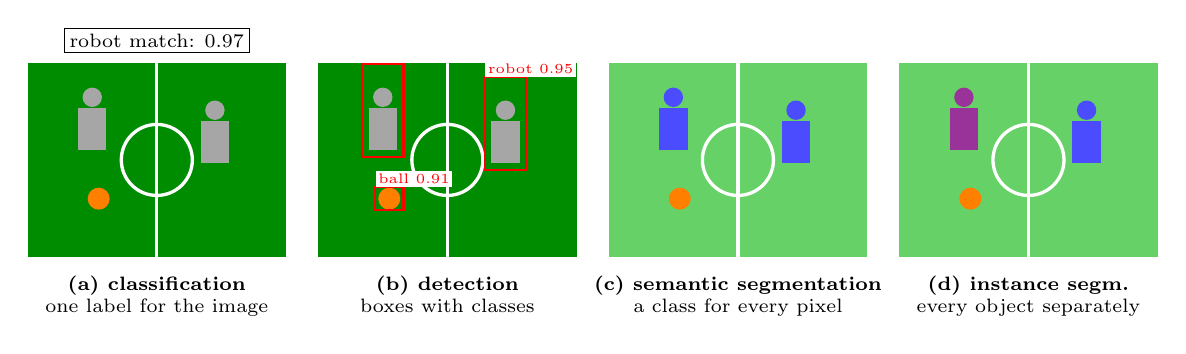
\begin{tikzpicture}[scale=0.82]
  \begin{scope}
    \scene{green!55!black}{white}{orange}{gray!70}{gray!70}
    \node[font=\scriptsize,align=center,anchor=north] at (2,-0.15) {\textbf{(a) classification}\\one label for the image};
    \node[font=\scriptsize,fill=white,draw,inner sep=2pt] at (2,3.35) {robot match: 0.97};
  \end{scope}
  \begin{scope}[xshift=4.5cm]
    \scene{green!55!black}{white}{orange}{gray!70}{gray!70}
    \draw[red,thick] (2.58,1.35) rectangle (3.22,2.78);
    \draw[red,thick] (0.68,1.55) rectangle (1.32,2.98);
    \draw[red,thick] (0.88,0.72) rectangle (1.32,1.08);
    \node[font=\tiny,red,fill=white,inner sep=1pt,anchor=south west] at (2.58,2.78) {robot 0.95};
    \node[font=\tiny,red,fill=white,inner sep=1pt,anchor=south west] at (0.88,1.08) {ball 0.91};
    \node[font=\scriptsize,align=center,anchor=north] at (2,-0.15) {\textbf{(b) detection}\\boxes with classes};
  \end{scope}
  \begin{scope}[xshift=9cm]
    \scene{green!70!black!60}{white}{orange}{blue!70}{blue!70}
    \node[font=\scriptsize,align=center,anchor=north] at (2,-0.15) {\textbf{(c) semantic segmentation}\\a class for every pixel};
  \end{scope}
  \begin{scope}[xshift=13.5cm]
    \scene{green!70!black!60}{white}{orange}{blue!70}{violet!80}
    \node[font=\scriptsize,align=center,anchor=north] at (2,-0.15) {\textbf{(d) instance segm.}\\every object separately};
  \end{scope}
\end{tikzpicture}
\captionof{figure}{Four vision tasks on a toy scene of a ball and two robots. Classification gives one label. Detection gives a box and a class for every object. Semantic segmentation colours every pixel by its class (grass, line, ball, robot). Instance segmentation also separates the individual robots.}\label{fig:ai1_vision}
\end{center}

\begin{itemize}[nosep]
  \item \textbf{Image classification:} ``what is in this image?'' The input is an image, the output is a list of probabilities, one per class, e.g.\ $(\text{ball}:0.94,\ \text{robot}:0.04,\ \text{other}:0.02)$. It cannot say \emph{where} the object is.
  \item \textbf{Object detection:} ``what is where?'' The output is a list of \textbf{bounding boxes}, each with a class and a confidence. This is what a robot needs to find the ball, the goal and other players. The YOLO models of Chapter~\ref{ch:ai4} belong here.
  \item \textbf{Semantic segmentation:} ``to which class does every pixel belong?'' The output is an image of class labels, with the same size as the input. It is the right tool for things without a clear box shape, such as the field lines, the grass or the free floor. All robots get the same label.
  \item \textbf{Instance segmentation:} like semantic segmentation, but every object gets its own label. (\textbf{Panoptic segmentation} combines both.)
\end{itemize}

More vision tasks: \textbf{pose estimation} (find the joints of a person or robot in the image), \textbf{tracking} (follow the same object over many frames), \textbf{depth estimation} (distance of every pixel), \textbf{optical flow} (how every pixel moves) and \textbf{text recognition} (OCR).

\section*{Other tasks}
Deep learning is far more than images:
\begin{itemize}[nosep]
  \item \textbf{Regression:} predict a number, such as the distance to the ball or the battery time that is left.
  \item \textbf{Time series:} predict or classify sequences of numbers, such as joint angles or IMU data (is the robot falling?).
  \item \textbf{Speech and audio:} speech recognition, detecting a whistle, speaker identification.
  \item \textbf{Language:} translation, summarising, question answering, writing code.
  \item \textbf{Anomaly detection:} find data that does not look normal (a motor that sounds unusual).
  \item \textbf{Recommendation:} suggest videos, songs, products.
  \item \textbf{Control and decision making:} choose actions in an environment (reinforcement learning, Part~VII).
\end{itemize}

\section*{Generative AI}
Most of the tasks above are \emph{discriminative}: they take data and produce a label, a box or a number. \textbf{Generative AI} creates \emph{new} data: text, images, speech, music, video or code. The model learns the distribution of the training data and then draws samples from it. The main families are:

\begin{center}
\renewcommand{\arraystretch}{1.3}
\begin{tabular}{p{3.3cm}p{6.2cm}p{4.6cm}}
\textbf{Family} & \textbf{Idea} & \textbf{Typical use}\\ \hline
Autoregressive models (large language models) & Predict the next piece (token), append it, repeat. & text, code, chat assistants\\
Generative adversarial networks (GAN) & A generator makes fakes, a discriminator tries to detect them; both improve. & realistic images\\
Variational autoencoders (VAE) & Compress data to a small code and decode it again; sample new codes. & images, compression\\
Diffusion models & Learn to remove noise step by step, then start from pure noise. & image, audio and video generation\\
\end{tabular}
\end{center}

For an autoregressive model the generation is a loop. For the beginning ``the robot kicks the'' the model computes a probability for every possible next token, for example ball $0.62$, goal $0.11$, \dots, picks one (usually a likely one) and continues. Chapter~\ref{ch:ai8} explains how this works. Generative models can \emph{make mistakes that sound very convincing} (``hallucinations''), so their output must be checked when it matters.

\begin{aibox}
In a robot team generative AI is useful for writing and reviewing code, for generating synthetic training images (a ball in many lighting conditions), and for talking to the robot in natural language. For the real-time control of the legs, small specialised networks trained with RL (Part~VII) are used.
\end{aibox}

\section*{Which method for which problem?}
\begin{center}
\renewcommand{\arraystretch}{1.3}
\begin{tabular}{p{5.6cm}p{3.6cm}p{5.0cm}}
\textbf{Problem} & \textbf{Method family} & \textbf{Why}\\ \hline
When the battery is low, go to the charger & rules & simple, must be 100\,\% reliable\\
Which of two actions is better, from a few numbers & decision tree & few data, explainable\\
Find groups in unlabelled sensor data & k-means & no labels needed\\
Where is the ball in the camera image? & detection network (YOLO) & images need deep learning\\
Which pixels are field lines? & semantic segmentation & a class for every pixel\\
Walk without falling & RL with a neural network policy & no ``right answer'', only a reward\\
Answer a question in natural language & large language model & generative text model\\
\end{tabular}
\end{center}

\section*{Practice problems}
\begin{enumerate}[label=\textbf{\thechapter.\arabic*}]
  \item Sort into ``symbolic AI'' or ``machine learning'': (a) a rule ``if the battery is below $10\,\%$ go to the charger'', (b) a classifier trained on $10\,000$ labelled images, (c) k-means on the colours of the pixels, (d) a Prolog program that answers who can pass to whom.
  \item Add the fact \texttt{free(clara).} to the Prolog program of this chapter. Which answers does the query \texttt{can\_pass(anna, Who).} give now?
  \item Compute the Gini impurity of (a) a group with $5$ ``shoot'' and $5$ ``pass'', (b) a group with $8$ ``pass'' and $2$ ``shoot'', (c) a group with only ``pass''.
  \item Classify with the decision tree of Figure~\ref{fig:ai1_tree}: (a) $d=2.8$\,m, no opponent, (b) $d=4.0$\,m, no opponent, (c) $d=1.2$\,m, opponent in front.
  \item Four points $(0,0)$, $(0,2)$, $(6,0)$, $(6,2)$ and two starting centres $c_1=(0,0)$, $c_2=(6,2)$. Perform one round of k-means (assign, then compute the new centres).
  \item An SVM has $\vv w=(\frac23,\frac23)$ and $b=-3$. (a) Which class (sign) do the points $(2,2)$ and $(4,4)$ get? (b) What is the distance of $(2,2)$ to the separating line? (Use $|\vv w\cdot\vv x+b|/|\vv w|$.) (c) How wide is the margin band?
  \item Which learning type is it? (a) $50\,000$ images with the label ``ball'' or ``no ball'', (b) the robot sorts $10\,000$ recorded motor sounds into groups without any labels, (c) $200$ labelled and $20\,000$ unlabelled frames from match videos, (d) a language model is trained to predict the next word of texts from the internet.
  \item Which vision task is needed? (a) Is a ball visible at all? (b) Where in the image is the ball? (c) Which pixels are the field lines? (d) Mark each robot with its own colour.
  \item A quadratic neuron computes $z=x_1x_2$. Compute $z$ for $(2,3)$, $(-1,4)$ and $(-2,-2)$ and give the class (sign).
  \item[\textbf{\thechapter.10}$\star$] A general quadratic neuron with $n$ inputs has $\frac{n(n+1)}{2}+n+1$ parameters. Compute the number for $n=10$ and $n=100$ and compare with an ordinary neuron. What does this tell you about using quadratic neurons for images?
\end{enumerate}
